\chapter{Einleitung}

\section{Motivation}

In der Literatur findet man viele verschiedene Definitionen eines verteilten Systems. Vieler dieser Definitionen unterschieden sich untereinander, so dass es schwer f�llt eine Definition zu finden, die als Alleinige als die Richtige gilt. Andrew Tanenbaum und Marten van Steen w\"{a}hlten f�r die Beschreibung eines verteilten Systems die folgende lockere Charakterisierung:

\cite{Tanenbaum} \textit{``Ein verteiltes System ist eine Menge voneinander unabh�ngiger Computer, die dem Anwender wie ein einzelnes, koh�rentes System erscheinen''}

Der Anwender muss sich nur mit dem lokalen, vor ihm befindlichen Computer auseinandersetzen, w�hrend die Software des lokalen Computers die reibungslose Kommunikation mit den anderen beteiligten Computern des verteilten Systems sicherstellt.

Diese Diplomarbeit soll den Anwendern die Betrachtung von verteilten Systemen aus einer anderen Perspektive erleichtern. Hierbei wird nicht die Sichtweise eines Endbenutzers eingenommen, sondern es sollen die Funktionsweisen von Protokollen und deren Prozesse in verteilten Systemen begreifbar gemacht und gleichzeitig alle relevanten Ereignisse eines verteilten Systems transparent dargestellt werden. 

Um dieses Ziel zu erreichen soll, insbesondere f\"{u}r Lehr- und Lernzwecke an der Fachhochschule Aachen, ein Simulator entwickelt werden. Mit dem Simulator sollen Protokolle aus den verteilten Systemen mit ihren wichtigsten Einflussfaktoren anhand von Simulationen nachgeblidet werden k\"{o}nnen. Gleichzeitig muss f�r eigene Experimente ein gro�er Spielraum zur Verf�gung stehen, wobei es keine Beschr�nkung auf eine feste Anzahl von Protokollen geben darf. Es ist also wichtig, dass es dem Anwender erm�glicht wird eigene Protokolle zu entwerfen.

\section{Grundlagen}

F�r das Grundverst�ndnis werden im Folgenden einige Grundlagen erl�utert. Eine Vertiefung findet erst in den sp�teren Kapiteln statt.

\subsubsection{Client/Server Modell}

\begin{figure}[htbp]
	\centering
	\fbox{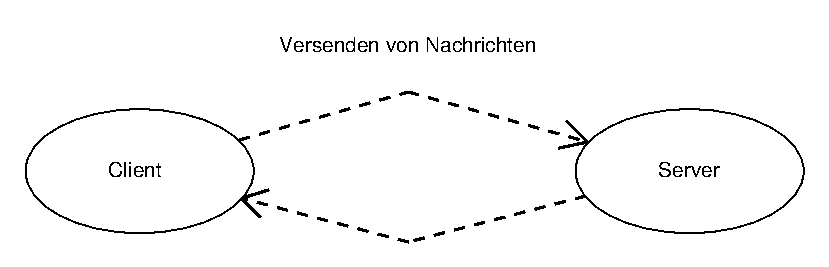
\includegraphics{images/client-server}}
	\caption{Client/Server Modell}
	\label{fig:ClientServer}
\end{figure}

Der Simulator basiert auf dem Client/Server-Prinzip. Jede Simulation besteht in der Regel aus einen teilnehmenden Client und einen Server, die miteinander �ber Nachrichten kommunizieren (s. Abbildung \ref{fig:ClientServer}.). Bei komplexen Simulationen k�nnen auch mehrere Clients und/oder Server mitwirken. 

\subsubsection{Prozesse und deren Rollen}

Ein verteiltes System wird anhand von Prozessen simuliert. Jeder Prozess nimmt hierbei eine oder mehrere Rollen ein. Beispielsweise kann ein Prozess die Rolle eines Clients einnehmen und ein weiterer Prozess die Rolle eines Servers. Die M\"{o}glichkeit einem Prozess die Client- und Serverrolle gleichzeitig zuzuweisen ist ebenso gegeben. Ein Prozess k\"{o}nnte auch die Rollen mehrerer Server und Clients gleichzeitig einnehmen. Um einen Prozess zu kennzeichnen besitzt, jeder eine \textbf{eindeutige} Prozess-Identifikationsnummer (PID). 

\subsubsection{Nachrichten}

In einem verteilten System m�ssen Nachrichten verschickt werden k�nnen. Eine Nachricht kann von einem Client- oder Serverprozess verschickt werden und kann beliebig viele Empf�nger haben. Der Inhalt einer Nachricht h�ngt vom verwendeten Protokoll ab. Was unter einem Protokoll zu verstehen ist, wird sp�ter behandelt. Um eine Nachricht zu kennzeichnen, besitzt jede Nachricht eine \textbf{eindeutige} Nachrichten-Identifikationsnummer (NID).

\subsubsection{Lokale und globale Uhren}

In einer Simulation gibt es \textbf{genau eine} globale Uhr. Sie stellt die aktuelle und \textbf{immer korrekte} Zeit dar. Eine globale Uhr geht nie falsch.

Zudem besitzt jeder beteiligte Prozess eine eigene lokale Uhr. Sie stellt die aktuelle Zeit des jeweiligen Prozesses dar. Im Gegensatz zu der globalen Uhr k�nnen lokale Uhren eine falsche Zeit anzeigen. Wenn die Prozesszeit nicht global-korrekt ist (nicht der globalen Zeit gleicht, bzw. eine falsche Zeit anzeigt), dann wurde sie entweder im Laufe einer Simulation neu gestellt, oder sie geht wegen einer Uhrabweichung falsch. Die Uhrabweichung gibt an, um welchen Faktor die Uhr falsch geht. Hierauf wird sp�ter genauer eingegangen. 

\begin{figure}[htbp]
	\centering
	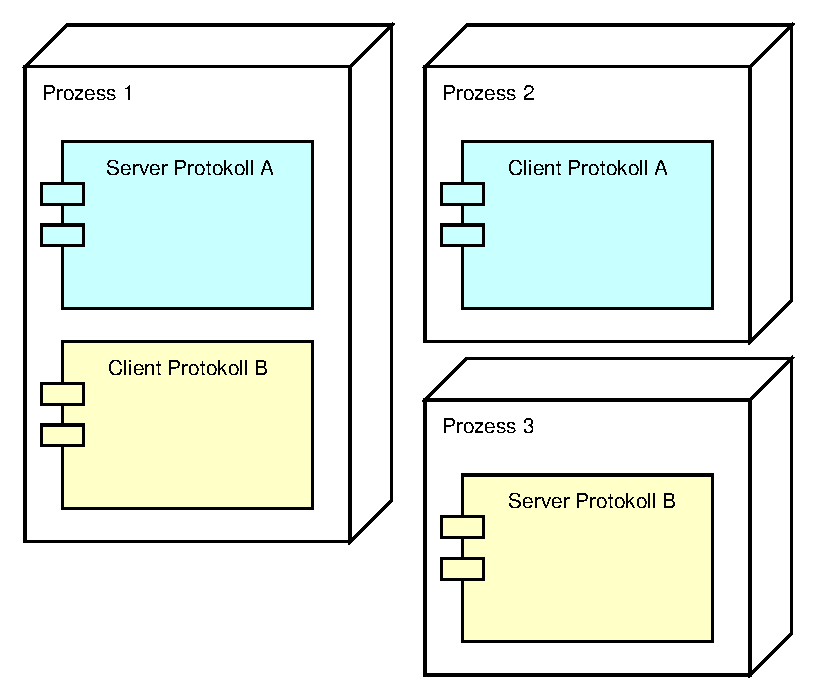
\includegraphics{images/client-server-protokolle}
	\caption{Client/Server Protokolle}
	\label{fig:ClientServerProtokolle}
\end{figure}

Neben den normalen Uhren sind auch die Vektor-Zeitstempel sowie die logischen Uhren von Lamport von Interesse. Jeder Prozess besitzt zus�tzlich einen Vektor-Zeitstempel f�r seine Vektorzeit, sowie einen Lamport-Zeitstempel f�r seine Lamportzeit. F�r die Vektor- und Lamportzeiten gibt es hier, im Gegensatz zu der normalen Zeit, keine globalen �quivalente. Konkrete Beispiele zu den Lamport- und Vektorzeiten werden sp�ter in Kapitel 3.11.1. behandelt.

\subsubsection{Ereignisse}

Eine Simulation besteht aus der Hintereinanderausf�hrung von endlich vielen Ereignissen. Beispielsweise kann es ein Ereignis geben, welches einen Prozess eine Nachricht verschicken l�sst. Denkbar w�re auch ein Prozessabsturzereignis. Jedes Ereignis tritt zu einem bestimmten Zeitpunkt ein. Ereignisse mit selber Eintrittszeit werden vom Simulator direkt hintereinander ausgef�hrt. Den Anwender des Simulators hindert dies jedoch nicht, da Ereignisse aus ihrer Sicht parallel ausgef�hrt werden.

\subsubsection{Protokolle}

Eine Simulation besteht auch aus der Anwendung von Protokollen. Es wurde bereits erw�hnt, dass ein Prozess die Rollen von Servern und/oder Clients annehmen kann. Bei jeder Server- und Clientrolle muss zus�tzlich das dazugeh�rige Protokoll spezifiziert werden. Ein Protokoll definiert, wie ein Client und ein Server Nachrichten verschickt, und wie bei Ankunft einer Nachricht reagiert wird. Ein Protokoll legt auch fest, welche Daten in einer Nachricht enthalten sind. Ein Prozess verarbeitet eine empfangene Nachricht nur, wenn er das jeweilige Protokoll versteht.

In Abbildung \ref{fig:ClientServerProtokolle}. sind 3 Prozesse dargestellt. Prozess 1 unterst�tzt serverseitig das Protokoll ``A'' und clientseitig das Protokoll ``B''. Prozess 2 unterst�tzt clientseitig das Protokoll ``A'' und Prozess 3 serverseitig das Protokoll ``B''. Das hei�t, dass Prozess 1 mit Prozess 2 via Protokoll ``A'' und mit Prozess 3 via Protokoll ``B'' kommunizieren kann. Die Prozesse 2 und 3 sind zueinander inkompatibel und k�nnen voneinander erhaltene Nachrichten nicht verarbeiten.

Clients k�nnen nicht mit Clients, und Server nicht mit Servern kommunizieren. F�r eine Kommunikation wird stets mindestens ein Client und ein Server ben�tigt. Diese Einschr�nkung kann aber umgangen werden, indem Prozesse ein gegebenes Protokoll sowohl server- als auch clientseitig unterst�tzen (vgl. Broadcast Protokoll in Kapitel 3.3.). 

